\section{Optimal Feature Selection Problem in SPL}\label{sec:problem}

In this section, we briefly introduce the optimal feature selection problem  and its formulation as a MOO problem.

%\subsection{Software Product Line}
%\label{spl}


\subsection{Feature Model and the Constraints inside}
\label{featuremodel}
%{\color{red}b.	Feature Models (an NP-hard problem to find) (Xue ge)}
In SE, \emph{feature} is defined as \lq\lq{}A distinguishing characteristic of a software item (e.g., performance, portability, or functionality)\rq\rq{} in \emph{IEEE Std} 829-1998.
In SPL,  \emph{feature} further refers to the requirements and implementations of such a characteristic \cite{tr:foda}. \emph{Feature model} is a hierarchy of the features within the product family as well as their structural and semantic (\emph{require} or \emph{exclude}) constraints in between \cite{DBLP:books/daglib/0010411}. %Feature model has even been regarded as \lq\lq the greatest contribution of domain engineering to software engineering{\rq\rq} \cite{DBLP:books/daglib/0010411}.

Feature model organizes the features inside in a tree-like structure. %The structural relationships between a parent (or compound) feature and its child features (or subfeatures) can be specified as:
Given a parent (or compound) feature $f^\prime$ and its child features (or subfeatures) \{$f_1,...,f_n$\}, four types of tree-structure constraints (TCs) exist and are defined as follow~\cite{DBLP:conf/splc/Batory05}:

\begin{itemize}[itemindent=*]
%\item \textit{And} -- If the parent feature is selected, all the sub-features should be also selected.
\item  $f_i$ is a \emph{mandatory} subfeature --- $f_i \Leftrightarrow f^\prime$,
%sometimes called \lq\lq Compulsory{\rq\rq}, referring to features that required \lq\lq And{\rq\rq}
\item  $f_i$ is an \emph{optional} subfeature --- $f_i \Rightarrow f^\prime$,
\item  \{$f_1,...,f_n$\} is an \emph{or} subfeature group ---  $f_1 \vee ... \vee f_n\Leftrightarrow f^\prime$,
\item  \{$f_1,...,f_n$\} is an \emph{alternative} subfeature group --- $(f_1 \vee f_2 \vee ... \vee f_n\Leftrightarrow f^\prime)\wedge \bigwedge\limits_{1 \le i<j\le n}(\neg(f_i \wedge f_j))$.
\end{itemize}

Given two features $f_1$ and $f_2$ that hold no TCs, three types of cross-tree semantic constraints  (CTCs) may exist, i.e.,\emph{iff}, \emph{requires} and \emph{excludes} \cite{DBLP:conf/splc/Batory05}:

\begin{itemize}[itemindent=*]
\item $f_1$ \emph{iff} $f_2$ --- $f_1 \Leftrightarrow f_2$,
\item $f_1$ \emph{requires} $f_2$ --- $f_1 \Rightarrow f_2$,
\item $f_1$ \emph{excludes} $f_2$ --- $\neg(f_1 \wedge f_2)$.
\end{itemize}

%
%\begin{itemize}
%%\item \textit{And} -- If the parent feature is selected, all the sub-features should be also selected.
%\item \textit{Alternative} -- If the parent feature is selected, exactly one among the exclusive subfeatures should be selected,
%\item \textit{Or} -- If the parent feature is selected, at least one of the subfeatures must be selected,
%\item \textit{Mandatory} -- A mandatory feature must be selected if its parent is selected,
%%sometimes called \lq\lq Compulsory{\rq\rq}, referring to features that required \lq\lq And{\rq\rq}
%\item \textit{Optional} -- An optional feature is optional to be selected.
%
%%features that are optional.
%\end{itemize}
%
%Besides the above structure or parental relationships between features, cross-tree constraints (CTCs) are also often adopted to represent the mutual relationship for features across the feature model. There are three types of common CTCs:
%
%\begin{itemize}
%\item $f_1$ \textit{requires} $f_2$ -- The inclusion of feature $f_a$ implies the inclusion of feature $f_b$ in the same product.
%\item $f_1$ \textit{excludes} $f_2$ -- The inclusion of feature $f_a$ implies the exclusion of feature $f_b$ in the same product, and vice versa.
%\item $f_1$ \textit{iff} $f_2$ -- The inclusion of feature $f_a$ implies the inclusion of feature $f_b$ in the same product, and vice versa.
%\end{itemize}
%

%Recently, to enhance the expressiveness, some work \cite{DBLP:journals/sopr/CzarneckiHE05} proposed to make \textit{Or} relationships with $[n:m]$  cardinalities, which more specifically denotes that a minimum of $n$ features and a maximum of $m$ features can be selected.


\begin{figure}[t]
\centering
\vspace{-1mm}
%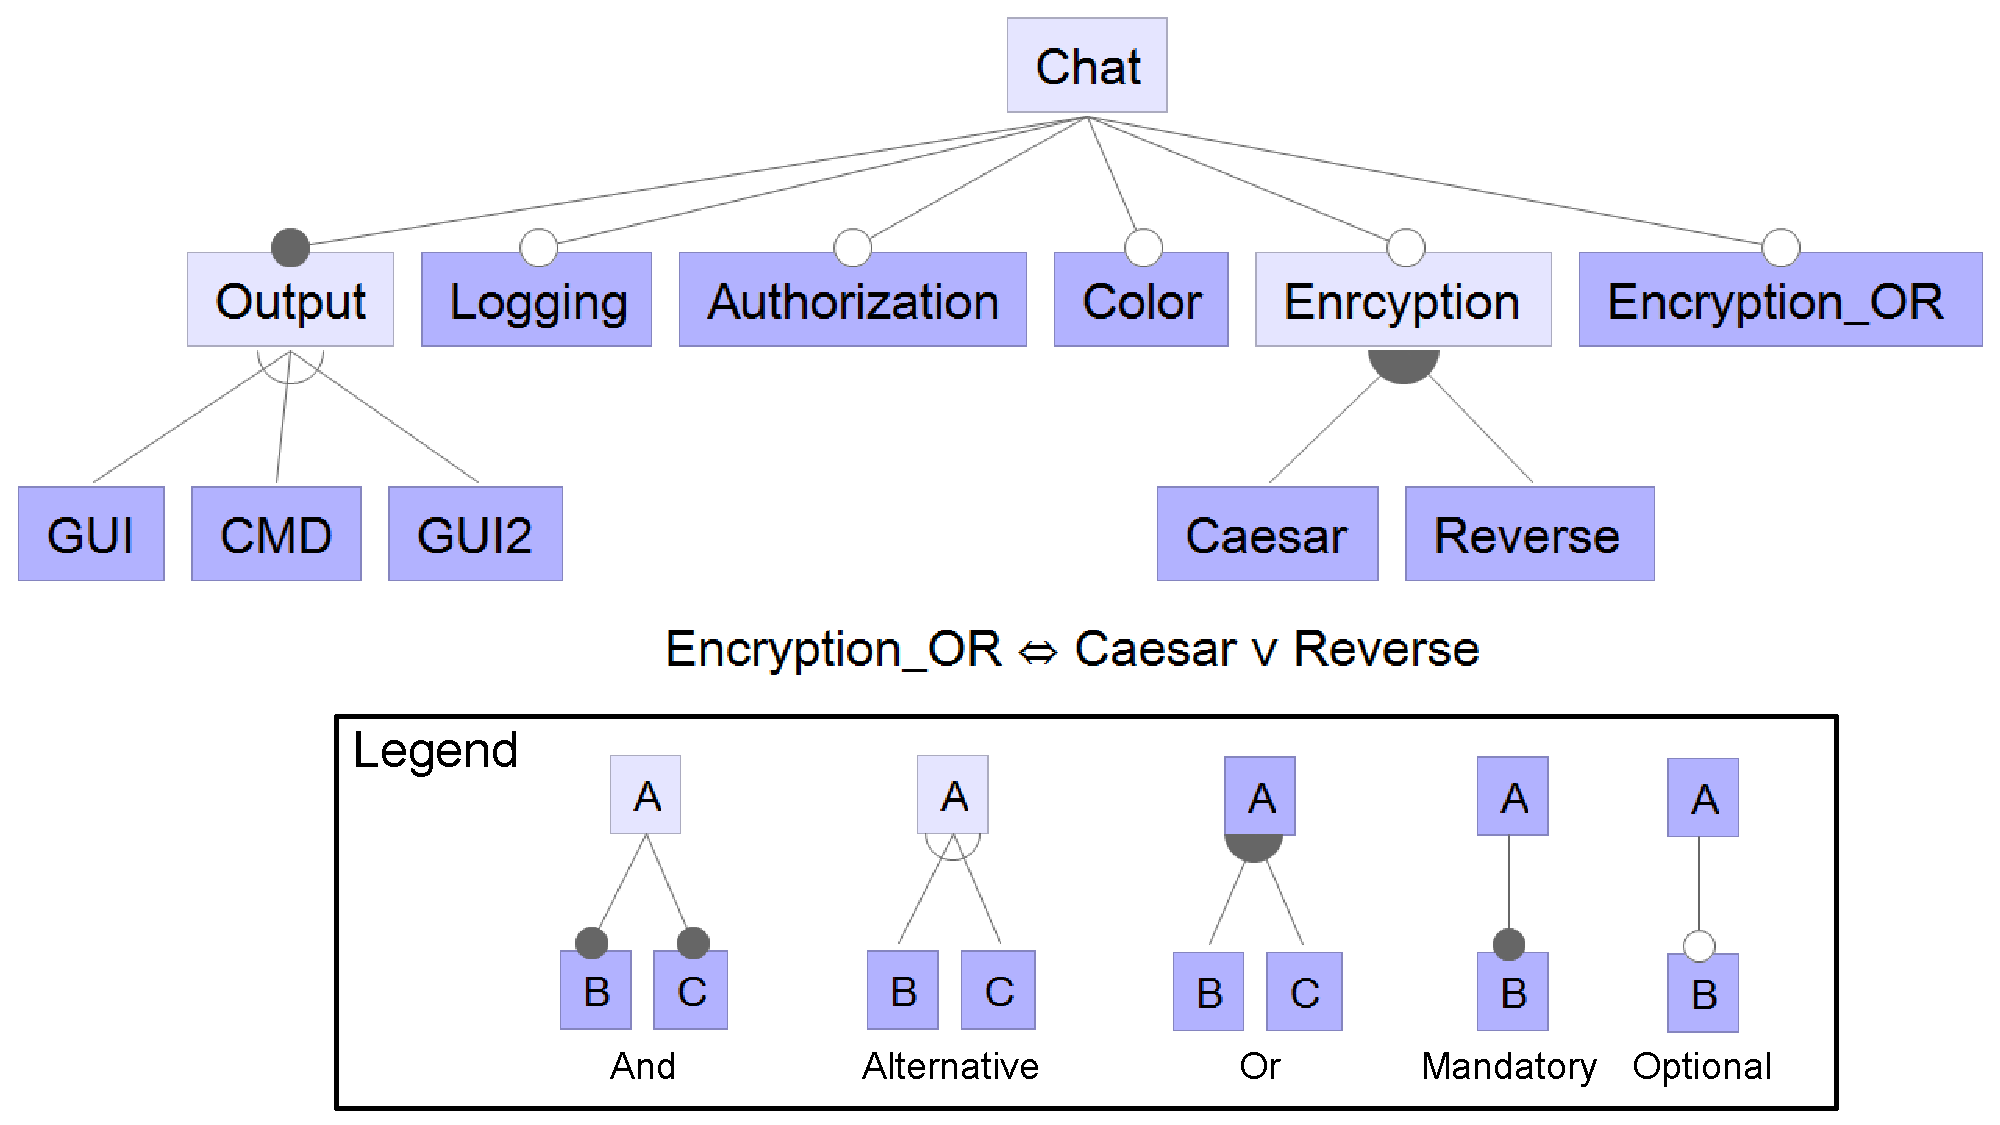
\epsfig{file=image/fm.bmp, width=8.5cm}
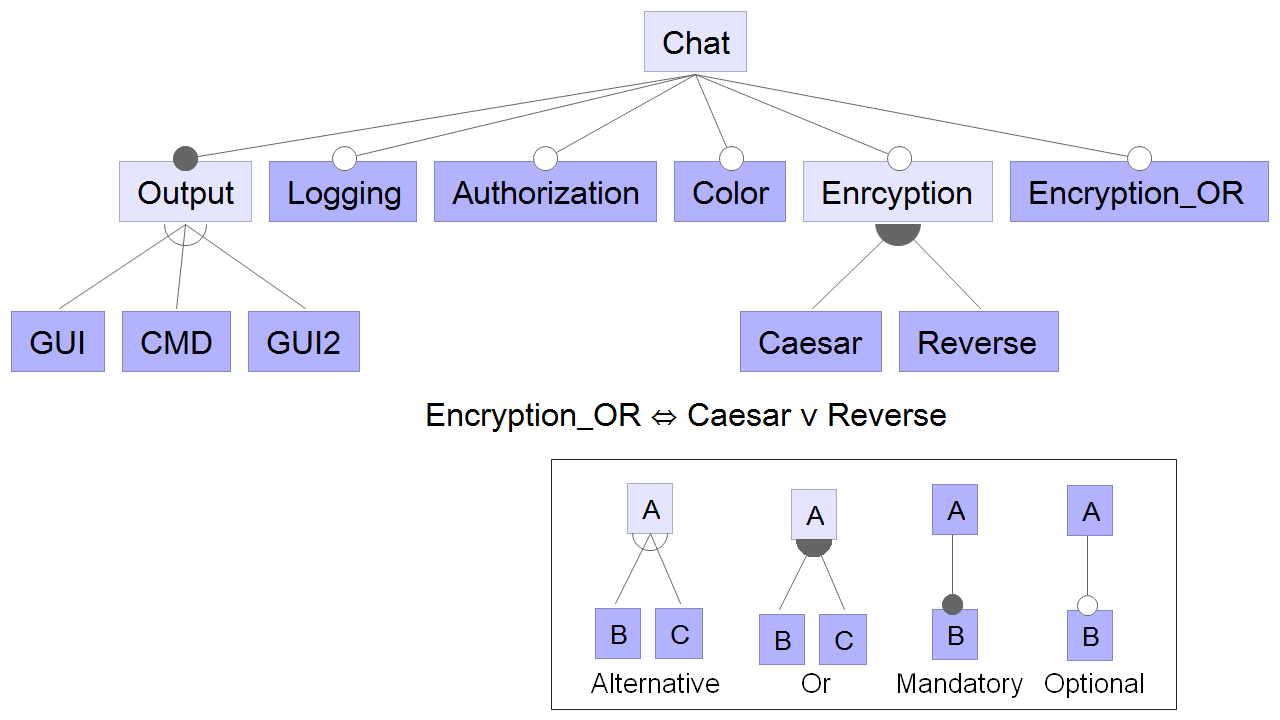
\includegraphics[width=8.5cm]{image/fm2.png}
\vspace{-2mm}
\caption{The feature model of $\JCS$ from \cite{DBLP:conf/issta/TanXCSLD15}}

\label{fig:re}
\end{figure}

The feature model of a Java Chat System ($\JCS$) is illustrated in Fig. \ref{fig:re} and the constraints of that model are listed in Table \ref{table:constrains}.
 Constraints c(1) -- c(12) are TCs, as they are constraints on structural relation of features. The root (compulsory) feature of the feature model is \textit{Chat}, which has a mandatory subfeature (\textit{Output}) and several optional subfeatures (e.g., \textit{Encryption}) --- constraints c(1) -- c(7). Since the feature \textit{Output}  is mandatory, exactly one of its subfeatures (\textit{GUI}, \textit{CMD}, and \textit{GUI2}) must be selected --- constraints c(8) -- c(11). In addition, if feature \textit{Encryption}  is selected, at least one of its subfeatures (\textit{Caesar} and \textit{Reverse}) needs to be selected --- constraints c(12). There is only one CTC for $\JCS$, which is of the form $f_1\ \mathit{iff}\ f_2$, \textit{Encryption\_OR} is selected if and only if \textit{Caesar} or \textit{Reverse} is selected ---  constraints c(13).

%The feature model listed in Fig. \ref{fig:re} can be captured by the constraints that are listed in~\mtable{table:constrains}. The constraints are specified according to the semantics of feature model.  %Constraint c(1) specifies that the root feature must be present, to prevent a trivial feature model with no selected feature. Constraint c(2) specifies the mandatory feature \textit{Output} and constraints c(3) -- c(7) specify constraints on the other five optional subfeatures. The subfeatures of \textit{Output} are in an \textit{Alternative} relationship. This is specified using constraints c(8) -- c(11). Constraint c(8) states that \textit{Output} is selected, if and only if at least one of \textit{CMD}, \textit{GUI} and \textit{GUI2} is selected. Constraints c(9) -- c(11) specify that at most one feature from \textit{CMD}, \textit{GUI} and \textit{GUI2} can be chosen. The subfeatures of \textit{Encryption} are in \textit{Or} relationship. The constraint c(12) denotes if \textit{Encryption} is selected, then at least one feature from \textit{Caesar} and \textit{Reverse} needs to be selected, and vice versa.
%The only CTC of $\JCS$ is captured in the constraint c(13).
Given a feature model \emph{M}, we refer TCs and CTCs of \emph{M} as  the conjunction of constraints of $M$, denoted by $\mathit{conj(M)}$. Let $\mathit{Fea(M)}$ denote the feature set of $M$. Thus, for the features in \emph{JCS}, we have $\mathit{Fea(JCS)} = \{\scriptsize{\mathit{Chat}, \mathit{Output}, \mathit{Logging}, \mathit{Authorization}, \mathit{Color}, \mathit{Encryption},} \\
\mathit{Encryption\_OR}, \mathit{GUI}, \mathit{CMD}, \mathit{GUI2}, \mathit{Caesar}, \mathit{Reverse}\}$.% and $\mathit{\vert Fea(JCS) \vert}$=12.

%Given a feature model $M$,
%a \emph{feature valuation} is a function
%$\FV : \mathit{Fea(M)} \rightarrow \{\mathit{true}, \mathit{false}\}$ mapping a boolean value to each feature in the feature set $\mathit{Fea(M)}$, where the true (resp., false) value denotes the presence (resp., absence) of the feature. Given a constraint $C$, $C[\FV]$ denotes the constraint obtained by replacing each feature $Fea(M)$ with $\FV(F)$ in $C$.


%We write $\FV \models C$, if $C[\FV]$ evaluates to true, otherwise we write $\FV \not\models C$.

%  In addition to the tree constrains, there might be inter-feature cross-tree constrains (CTCs) like \textit{requires}, \textit{excludes} or \textit{iff}. In Figure \ref{fig:re}, below the feature model is a \textit{iff} type of CTCs c(12).

%In a feature model, a place that allows the flexible feature selection is called a variation point (VP) \cite{DBLP:conf/icsr/WebberG02}\cite{DBLP:conf/icse/JarzabekZLXS09}. The VP of a optional feature allows two options. The VP of an alternative relation of $n$ subfeatures allows $n$ options, while the VP of an or relation of $n$ subfeatures allows the options $C_{n}^{n} + C_{n}^{n-1}+ ...+ C_{n}^{1}$. Besides,

%A product derived from the feature model in Figure \ref{fig:re} must satisfy all constraints in Table \ref{table:constrains}. Therefore, finding a valid product derivation from a feature model can be reduced to a satisfaction problem on a set of logic formulas, also a NP-complete problem \cite{DBLP:journals/jss/WhiteDS09}. If the user preference values (extra non-functional constrains) are considered, finding an optimal product is shown to be NP-hard \cite{DBLP:conf/icse/SayyadMA13}. %\tth{Maybe just use a reference mentions that our work is NP-hard}

\vspace{-1mm}
\begin{myDef} [Correct  Solution]
Given a feature model $M$,  a \emph{correct solution}   for $M$ refers to a non-empty feature set $F \subseteq Fea(M)$ that satisfies the constraints of $M$.
\end{myDef}
\vspace{-1mm}

%We write $F \models M$ if $F \subseteq Fea(M)$ is a feasible feature set of the feature model $M$.
%\paratitle{Example}  We use
Take $\JCS$ as an example, $F=\{\mathit{Chat},\mathit{Output}, \mathit{GUI}\}$ is a correct solution of feature selection for $\JCS$. %Hence, an optimal feature selection must be a correct feature selection, and meanwhile, it optimizes several goals of product configuration.


%{\color{red} do you want to introduce the grammar of FM in this subsection or in the approach: the propositional logics for the semantic and constrains in FM?}

%Figure \ref{fig:re} shows the feature model of an SOSPL for online flight booking systems. This SOSPL can derive the different online flight booking system as a coarse-grained service to a different user. The \textit{abstract feature} in Figure \ref{fig:re} means this feature requires no specific implementation (thus, no need to be bound to a specific service), as an abstract feature usually is only a wrap of its sub-features. The \textit{concrete feature} means it has a specific function to perform, and it needs to be bound to a service to implement such function. Thus, in a valid product from this SOSPL, the selected concrete features must be bound to some services. Under the feature diagram in Figure \ref{fig:re}, the cross tree constrains of this FM are also listed.


\begin{table}[t]
\centering
\caption{Constraints of $\JCS$}
\vspace{-2mm}
\scalebox{0.9}{
\begin{tabular}{l|r}
\hline
$\mathit{Chat}$ & c(1)\\
$\mathit{Output} \iff  \mathit{Chat}$ & c(2)\\
$\mathit{Logging} \implies \mathit{Chat}$ & c(3)\\
$\mathit{Authorization} \implies \mathit{Chat} $ & c(4)\\
$\mathit{Color}\implies \mathit{Chat}$ & c(5)\\
$\mathit{Encryption}\implies \mathit{Chat}$ & c(6)\\
$\mathit{Encryption\_OR}\implies \mathit{Chat}$ & c(7)\\
$(\mathit{GUI} \lor \mathit{CMD} \lor \mathit{GUI2})\iff \mathit{Output}$ & c(8)\\
$\lnot(\mathit{GUI}\land \mathit{CMD})$ & c(9)\\
$\lnot(\mathit{GUI}\land \mathit{GUI2})$ & c(10)\\
$\lnot(\mathit{CMD}\land \mathit{GUI2})$ & c(11)\\
$(\mathit{Caesar}\lor \mathit{Reverse})\iff \mathit{Encryption}$ & c(12)\\
$\mathit{Encryption\_OR}\iff  (\mathit{Caesar} \lor \mathit{Reverse})$ & c(13)\\
\hline
\end{tabular}
}
%\vspace{-2mm}
\label{table:constrains}
\end{table}

\vspace{-1mm}
\subsection{Multi-objective Optimization for SPL}\label{sec:background:mop}
%Many real-world problems have multiple objectives that need to be optimized simultaneously. However, these objectives usually conflict with each other, which prevents optimizing all objectives simultaneously. A remedy is to have a set of optimal trade-offs between the conflicting objectives.

%A $k$-objective optimization problem could be written in the following form:
%\begin{equation}\label{eq:min}
%\begin{split}
%\emph{Minimize}\ Obj(F)=(Obj_1(F), Obj_2(F),..., Obj_k(F))\ \\  \emph{subject}\ \emph{to}\ F \models M
%\end{split}
%\end{equation}
%
% \noindent where $Obj(F)$ is a $k$-dimensional objective vector for $F$ and  $Obj_i(F)$ is the value of $F$ for $i$th objective.
%
%
%  Given $F_1, F_2 \models M$, $F_1$ can be viewed as better than $F_2$ for the minimization problem in~\mequation{eq:min}, if~\mequation{eq:minbetter} holds.
%
%A $k$-objective optimization problem could be written in the following form~\cite{abraham2005evolutionary}:
%\begin{equation}\label{eq:min}
%\emph{Minimize}\ f(x)=(f_1(x), f_2(x),..., f_k(x))\  \emph{subject}\ \emph{to}\ x \in X
%\end{equation}
%
%\noindent where $f(x)$ is a $k$-dimensional objective vector, and  $f_i(x)$ is the $i$th objective to be minimized, $x$ is the decision vector, and $X$ is the feasible region in the decision space.
%
%Consider $y$ and $z$ as two feasible solutions of the $k$-objective optimization problem in~\mequation{eq:min}, $y$ can be viewed as better than $z$ for the minimization probelm in~\mequation{eq:min}, if~\mequation{eq:minbetter} holds.

%\begin{equation}\label{eq:minbetter}
%\forall i: Obj_i(F_1) \leq Obj_i(F_2) \land \exists j: Obj_j(F_1) < Obj_j(F_2)
%\end{equation}
%
%\noindent  where $i,j \in \{1, \ldots, k\}$.
%
%In such a case, we say that $F_1$ \emph{dominates} $F_2$.  $F_1$ is called a \emph{Pareto-optimal solution} if $F_1$ is not dominated by any other $F \models M$. We denote all Pareto-optimal solutions as the \emph{Pareto front}.


%
% Assume $\textbf{y}$ and $\textbf{z}$ are two feasible solutions of the $k$-objective optimization problem, $\textbf{y}$ \emph{dominates} $\textbf{z}$ if $\forall i: f_i(\textbf{y}) \le f_i(\textbf{z})$ and $\exists j: f_j(\textbf{y}) < f_j(\textbf{z})$ where $i,j \in [1,k]$~\cite{DBLP:conf/gecco/IshibuchiTSN10}.
%
%
% $\textbf{y}$ is a \emph{Pareto-optimal solution} if $\textbf{y}$ is not dominated by any other feasible solutions. All Pareto-optimal solutions form the tradeoff space in the objective space, we denote the tradeoff space as the \emph{Pareto front}.


%To serve as the goals of malware generation, we propose three objective functions in the evolution of malware: \emph{aggressiveness}, \emph{evasiveness} and \emph{detectability}. As the results of the arms race, malware are getting more aggressive with minimum evasion features needed, but less detectable.
\subsubsection{Software Development Model and the Objectives}
As the correct selection of a non-empty feature set $F$ on feature model $M$ is essentially a boolean satisfiability (SAT) problem that attracted attention from researchers \cite{DBLP:conf/pfe/MannionC03}\cite{DBLP:conf/caise/BenavidesTC05}. %Insofar, many techniques have been applied to address this problem, such as theorem proving \cite{DBLP:conf/pfe/MannionC03}, Constraint Satisfaction Problems (CSP)~\cite{DBLP:conf/caise/BenavidesTC05} and OWL DL~\cite{DBLP:journals/ws/WangLSZP07}.
Gradually, this problem evolves into a MOO problem --- more than having a correct selection, multiple quality attributes of the product  generated according to $F$ need to be  optimized .

According to \cite{DBLP:journals/misq/Abdel-HamidSS99}, goals in software development indeed have a positive impact for the products. Project managers control the software development according to four objective scores: project risk; development cost, development defects; and manpower (total months of development)~\cite{DBLP:journals/misq/Abdel-HamidSS99}. %During product configuration for certain customers, project managers also consider other goals such as the richness of features and cost \cite{DBLP:conf/icse/SayyadMA13}.
According to \cite{DBLP:conf/icse/SayyadMA13}, each feature %(also with its relevant implementation module) in the feature model
is associated with three attributes, i.e., COST, DEFECT and USED\_BEFORE. The optimal feature selection problem can be ideally modeled as a MOO problem, which requires trade-off among multiple design goals.

\subsubsection{Formalization of the MOO Problem}\label{sec:problem:moo}

  Given a non-empty feature set $F$ and the entire feature set $Fea(M)$ for $M$ ($Fea(M) =\{f_1 ... f_n\}$. For  $ \forall f_i \in Fea(M)$, the binary value represented by the selection of $f_i$ (denoted as $|f_i|$) is \textbf{1} if $f_i \in F$, else $|f_i|$ is  \textbf{0}. Given a solution $\vec x$ (an encoded binary-value vector for $Fea(M)$),  we define objective functions as:

%\footnote{For the sake of simplicity and ease of evaluation, we use the five objectives defined in \cite{DBLP:conf/icse/SayyadMA13} for problem statement and evaluation.}
\begin{enumerate}[label=\textbf{Obj\arabic*.},itemindent=*]
  \item \textbf{Correctness} means the extent of the compliance to $conj(M)$. We want to minimize the number of violated constraints:  $\mathcal{F}_1(\vec x) = Viol(F)$, where $Viol(F)$ returns the number of constraints violated by $F$ among $conj(M)$. Note that $Viol(F)$ = 0 means a  correct selection.
  \item  \textbf{Richness of features} means the richness of the functionality of the product. We want to minimize the number of deselected features: $\mathcal{F}_2(\vec x) = \sum\nolimits_{i=1}^{n} (1-|f_i|)$, where $|f_i|$ returns 1 if $f_i \in F$, otherwise returns 0.
  \item   \textbf{Feature used before} means the reliability of product, as features never used are more prone to have unknown defects. We want to minimize this:
      $  \mathcal{F}_3(\vec x) = \sum\nolimits_{i=1}^{n} (Used(f_i)  \cdot  |f_i|)$, where $Used(f_i)$ returns a boolean value of the attribute USED\_BEFORE of feature $f_i$.
   \item \textbf{Defects} means the known bugs or errors contained in the product. We want to minimize this: %It can be quantified by the $
       $\mathcal{F}_4(\vec x) =  \sum\nolimits_{i=1}^{n}( Defect(f_i)   \cdot  |f_i|)$, where $Defect(f_i)$ returns the value of attribute DEFECT of feature $f_i$.
  \item  \textbf{Cost} means the expense and efforts in developing the product. We want to minimize this: $\mathcal{F}_5(\vec x) = \sum\nolimits_{i=1}^{n}( Cost(f_i)  \cdot   |f_i|)$, where  $Cost(f_i)$ returns the value of the attribute COST of feature $f_i$.
\end{enumerate}

%\vspace{-2mm}
%\begin{myDef}\label{def:aggressivity}
% \textbf{Correctness} means the extent of compliance to the relationships and constraints contained in the feature model, and can be formally defined as follow %such as privacy leakage, resource depletion, or controlled as a bot.  and the set of selected attack features $S_a$, aggressivity $f_1(x)$ is defined as follows:
%     \begin{equation}
%       \mathcal{F}_1(x) = Corr(F)
%         \end{equation} where $Corr(F)$ returns the number of violated constraints of $F$ among all the constraints of $M$\footnote{Note that $Corr(F)$ = 0 means that $F$ produces a correct feature selection.}.
%         %It can be measured by  the number of attack features contained in malware.
%       %It can be quantified by the number of contained attack features.
%\end{myDef}
%\vspace{-2mm}
%\vspace{-2mm}
%\begin{myDef}\label{def:complexity}
%\textbf{Richness of features} means the richness of the functionality of the product. It is measured by the number of selected features and defined as follows
%        \begin{equation}
%         \mathcal{F}_2(x) = \sum\nolimits_{i=1}^{n} \|f_i\|
%           \end{equation} where $\|f_i\|$ returns 1 if $f_i$ is selected and returns 0 if not.
%        %It can be measured by the number of evasion features used by malware. %It can be quantified by the number of used evasion features.\
%\end{myDef}
%\vspace{-2mm}
%
%%Given a chromosome $x$ and the set of AMTs $S_d$, $\{d_1...d_t\}$, introduced in Section \ref{sec:defense}, we have the following definition for the last objective function:
%
%\begin{myDef}\label{def:complexity}
%\textbf{Cost} means the expense and efforts in developing the product. It is an aggregate value and defined as follows
%        \begin{equation}
%         \mathcal{F}_3(x) = \sum\nolimits_{i=1}^{n}( Cost(f_i) \cdot   \|f_i\|)
%           \end{equation} where  $Cost(f_i)$ returns the value of the attribute COST of feature $f_i$.
%        %It can be measured by the number of evasion features used by malware. %It can be quantified by the number of used evasion features.\
%\end{myDef}
%\vspace{-2mm}
%
%\begin{myDef}\label{def:complexity}
%\textbf{Feature used before} means the reliability of product, as the features never used are more prone to contain unknown defects. It is an aggregate value and defined as follows
%        \begin{equation}
%         \mathcal{F}_4(x) = \sum\nolimits_{i=1}^{n} (Used(f_i)  \cdot  \|f_i\|)
%           \end{equation} where $Used(f_i)$ returns the boolean value of the attribute USED\_BEFORE of feature $f_i$.
%        %It can be measured by the number of evasion features used by malware. %It can be quantified by the number of used evasion features.\
%\end{myDef}
%\vspace{-2mm}
%
%\vspace{-2mm}
%\begin{myDef}\label{def:detectability}
% \textbf{Defects} means the bugs or errors contained in the product. It is an aggregate value and defined as follows  %It can be quantified by the detection ratio by different malware detection tools.
%       \begin{equation}
%       \mathcal{F}_5(x) =  \sum\nolimits_{i=1}^{n}( Defect(f_i)  \cdot  \|f_i\|)
%       \end{equation} where $Defect(f_i)$ returns the value of attribute DEFECT of feature $f_i$.
%\end{myDef}
%\vspace{-2mm}

%\subsubsection{Generation Steps}
%\vspace{-2mm}

%Since DSA capture the essence of malicious behaviors (see Chapter~\ref{sec:model}), we first construct basic malicious behaviors in terms of these DSA, then instrument communication mechanisms existing in Android to the malicious behaviors, and last employ obfuscation techniques to instrument the malware. The malware is sent to the module of risk assessment, which can give its fitness. The process is iterative and the malware evolves according to the fitness feedback. In this chapter, we elaborate the steps of malware generation.

%In this section, we introduce the algorithm to select the features, and improve the feature combination according to the evaluation of generated apps.

Rather than encode all the objectives into one magic weighted fitness function, all the objectives are equally treated and solved by MOO using the Pareto dominance relation~\cite{mopsurvey2008}.


A $k$-objective optimization problem could be written in the following form %\footnote{\small Evasiveness and detectability need to be minimized, but aggressiveness needs to be maximized. In implementation, maximizing is minimizing the negative value of the objective.}
(in our case, $k = 5$):
\begin{equation}\label{eq:min}
\begin{split}
\emph{Minimize}\ \mathcal{\vec F}=(\mathcal{F}_1(\vec x), \mathcal{F}_2(\vec x),..., \mathcal{F}_k(\vec x))\ \\ % \emph{subject}\ \emph{to}\ F \models M
\end{split}
\end{equation}
\noindent where $\mathcal{\vec F}$ is a $k$-dimensional objective vector and  $\mathcal{F}_i(\vec x)$ is the value of $\mathcal{\vec F}$ for $i$-th objective.
\begin{myDef}
Given two correct solutions $\vec x, \vec y \in B^n$ and an objective vector $ \mathcal{\vec F}: B^n \rightarrow R^k$, $\vec x$ \textbf{dominates} $\vec y$ ($ \vec x \prec \vec y$) if
    \begin{equation}
    \begin{split}
  \forall i \in \{1,...,k\} \quad \mathcal{F}_i(\vec x) \le \mathcal{F}_i(\vec y)
  \end{split}
     \end{equation}
    \begin{equation}
     \begin{split}
   \exists j \in \{1,...,k\} \quad \mathcal{F}_j(\vec x) < \mathcal{F}_j(\vec y)
     \end{split}
   \end{equation}
otherwise $\vec x \not\prec \vec y$
\end{myDef}
\vspace{-2mm}

\vspace{-2mm}
\begin{myDef}
Given a correct solution $\vec x$ and a set of correct solutions $S_{\vec x}$, $\vec x$ is \textbf{non-dominated} iff
      \begin{equation}
  \forall \vec x_i \in S_{\vec x} \quad \vec x_i \not\prec \vec x
       \end{equation}
\end{myDef}
\vspace{-2mm}
$\vec x$ is called a \emph{Pareto optimal} solution if $\vec x$ is \emph{correct} and \emph{not dominated} by any other correct solutions. All Pareto-optimal solutions are called as the true Pareto front.

\subsubsection{Problem Statement}

%\paratitle{Problem statement}
Existing MOEAs (e.g., IBEA~\cite{DBLP:conf/ppsn/ZitzlerK04}, NSGA-II~\cite{DBLP:journals/tec/BradstreetWB08}, ssNSGA-II~\cite{coello2004applications}, MOCell~\cite{miettinen1999nonlinear}, SPEA2 \cite{Zitzler01spea2:improving})  are used to find a set of non-dominated solutions that approximate the Pareto front for solving the MOO problems. %According to \cite{DBLP:conf/icse/SayyadMA13}, among them, NSGA-II and SPEA2 are most widely used in SBSE. For the optimal feature selection problem,
As pointed by Sayyad \emph{et.al} in \cite{DBLP:conf/icse/SayyadMA13}, IBEA produces the solutions with the highest correctness rate. After that, more studies improve IBEA to search for correct solutions \cite{conf/cmsbse/SayyadMA13}\cite{DBLP:conf/issta/TanXCSLD15}\cite{DBLP:conf/icse/HenardPHT15}\cite{DBLP:journals/tosem/HieronsLLSZ16}\cite{DBLP:journals/asc/XueZT0CC016}.

%However, whatever MOEA is used, the completeness of the found solutions and the quality of the approximated Pareto front cannot be guaranteed.

%\paratitle{Motivation}
%Our work addresses the \emph{optimal feature selection}. Nevertheless,
 As these MOEA-based approaches suffer from the correctness, %we treat this optimal feature selection problem as a mix of SAT and MOO problem ---  assure the solutions are correct solutions (i.e., assuring $Vio(F)=0$) and then optimize the other four objectives.
why not we use a method naturally assuring the solution correctness?   As all constraints in $conj(M)$  and all objectives are \emph{linear} (convertible to linear inequalities, see \S\ref{sec:formulate}),  Binary Integer Programming (BIP) can be applied. In theory, we can reduce the multiple objectives into one. The BIP-based analytic method is free from the drawbacks of MOEAs (see \S\ref{sec:intro}), but may suffer from the scalability issue. %In \S\ref{sec:naiveSolutions} and \S\ref{sec:solution}, we reduce multi-objective to one for applying LP.

%it is \xyx{Inspired by [??], we aim to design an analytic approach that solve the subproblem of satisfiability and  optimisation subproblem  in polynomial time. }

 %, such as Genetic Algorithms, Evolutionary Strategies and Differential Evolution.

%We use the Indicator-Based Evolutionary Algorithm (IBEA)~\cite{DBLP:conf/ppsn/ZitzlerK04}, which has already been implemented in the jMetal framework~\cite{DBLP:journals/aes/DurilloN11}.
%\subsection{Problem Statement}


%Given multiple objectives to be optimized, we have the following definition:

%\begin{definition} [optimal feature set]
%Given a feature model $M$,  an \emph{optimal feature set} for $M$ is a feasible feature set $f \models M$, which is not dominated by any feasible feature set $f' \models  M$, where $f \neq f'$.
%\end{definition}

%\begin{definition}[optimal feature selection]
%Given a feature model $M$,  an \emph{optimal feature selection} is a set of optimal feature sets of $M$.
%\end{definition}
%\emph{Optimal feature selection} of feature model $M$ is to select a set of optimal features sets for $M$.

%Our work addresses \emph{optimal feature selection}, which aims to search for a feasible feature sets that approximate the Pareto
%front for solving the multi-objective optimization problem.

%We denote the \emph{size} of optimal feature selection $S$ as the number of optimal feature sets in $S$.

%In addition, given two EAs $ea_1$ and $ea_2$, we say that $ea_1$ provides an improvement than $ea_2$ in finding an optimal feature selection, if the size of the optimal feature selection found by $ea_1$ is strictly larger than $ea_2$.

%\paratitle{Example} We use $\JCS$ as an example. Suppose we want to minimize the cost of the feature selection, and all features are free, except features $\mathit{GUI}$ comes with a cost. In this case, $f=\{\mathit{Chat},\mathit{Output},\mathit{GUI}\}$ is a feasible feature selection, but it is not an optimal feature selection. This is because $f$ is dominated by, for example $\{\mathit{Chat},\mathit{Output},\mathit{CMD}\}$, which has lower cost. Both $o_1=\{\mathit{Chat},\mathit{Output},\mathit{CMD}\}$ and $o_2=\{\mathit{Chat},\mathit{Output},\mathit{GUI2}\}$ are optimal feature sets, and $\{o_1, o_2\}$ is an optimal feature selection, with size of 2.

